\subsection{Mudanças resultantes da avaliação}
\label{sec:mudanasresultantes}

Considerando as principais dificuldades relatadas pelos usuários da DSL Cotas, nessa Subseção são descritas as melhorias implementadas na linguagem que foram selecionadas com o objetivo de reduzir as lacunas de entendimento sobre a distribuição das vagas e também melhorar a clareza das mensagens de erros e avisos aos usuários.

A primeira melhoria é a responsável pelo tratamento das sugestões apontadas pelos usuários do grupo DEV-ESP e NDEV-ESP, os quais relataram a necessidade de visualização prévia de simulação das vagas. Para tanto, foi adicionado um novo elemento do tipo \texttt{behavior}, \texttt{Distribuicao\_Behavior} no qual foram inseridos métodos para varrer a \gls{AST} e fazer os cálculos do quadro de vagas seguindo as definições preenchidas pelo usuário da DSL (Código Fonte \ref{lst:distribuicao_behavior}).

\newpage

\lstinputlisting[language=Java, 
caption=Behavior para cálculo do quadro de vagas 
,label=lst:distribuicao_behavior]{chapters/trechos_codigo/distribuicao_behavior.m}


O método \texttt{calculaDistribuicao} (Linha 3) acessa a \texttt{CategoriaCota} raiz, o valor de simulação desejado e a forma de arredondamento definida pelo usuário, e em sequência, por meio do método recursivo \texttt{calculaVagasCategoria} (Linha 14) são realizadas iterações em todas as categorias subsequentes da distribuição, calculando as vagas conforme os respectivos percentuais (Linha 24) ou fazendo o cálculo de soma das vagas para a constante \texttt{RESTANTE\_VAGAS} (Linha 27). 

Os números de vagas para cada categoria são armazenados em um novo atributo do conceito, nomeado de \texttt{numeroVagas}, esses valores são atualizados sempre que o usuário aciona a função de simulação na DSL ou no caso da forma de arredondamento ser alterada. Desse modo, foi possível adicionar novos elementos no editor dos conceitos \texttt{CategoriaCota} e \texttt{Distribuicao} para apresentar o valor calculado, além de gerar uma listagem do quadro de vagas (Figuras \ref{fig:editoralterado}, \ref{fig:simulacaovagas} e \ref{fig:quadrosimulacao}).


\begin{figure}[ht!]
\centering

\caption{\textmd{Editores alterados para simulação de vagas}}
\label{fig:editoralterado}
\fcolorbox{gray}{white}{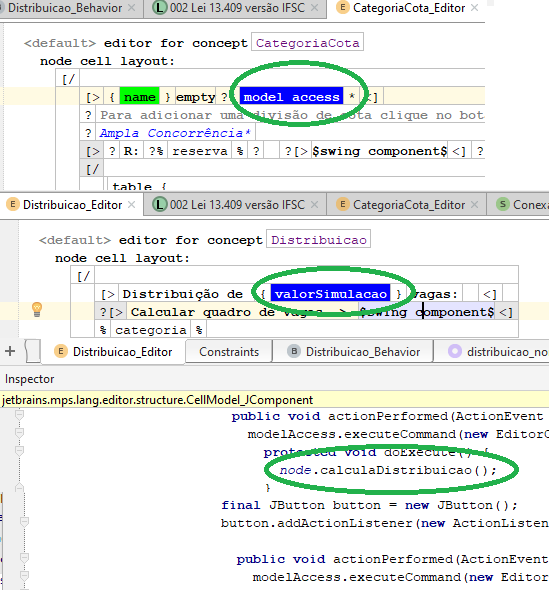
\includegraphics[width=0.65\textwidth]{chapters/analise/imagens/editoralterado.png}}

\par\medskip\textbf{Fonte:} Elaborado pelo autor (2020). \par\medskip

\caption{\textmd{Simulação de vagas durante a definição da distribuição}}
\label{fig:simulacaovagas}
\fcolorbox{gray}{white}{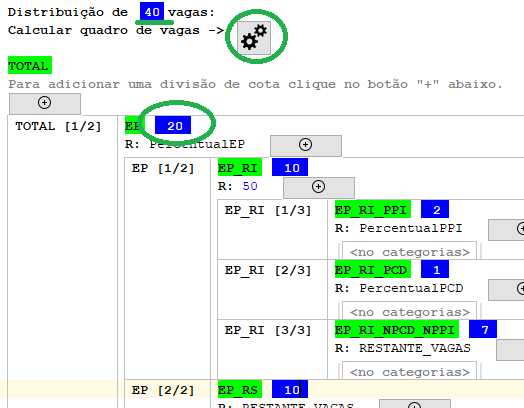
\includegraphics[width=0.75\textwidth]{chapters/analise/imagens/simulacaovagas.png}}

\par\medskip\textbf{Fonte:} Elaborado pelo autor (2020). \par\medskip

\end{figure}



\clearpage
\begin{figure}[ht!]
\centering

\caption{\textmd{Simulação do quadro de vagas}}
\label{fig:quadrosimulacao}
\fcolorbox{gray}{white}{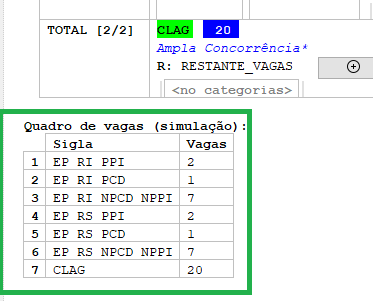
\includegraphics[width=0.55\textwidth]{chapters/analise/imagens/quadrosimulacao.png}}

\par\medskip\textbf{Fonte:} Elaborado pelo autor (2020). \par\medskip

\end{figure}




A visualização prévia dos cálculos pode auxiliar no entendimento dos requisitos de distribuição de vagas para todos os grupos de usuários analisados, possibilitando que tenham uma simulação imediata dos elementos da linguagem, além de auxiliar no caso de dúvidas sobre como os percentuais são aplicados no contexto da árvore de distribuição.

Com relação às dificuldades de entendimento das mensagens de erro e dos avisos apresentados pela linguagem, foram alteradas as instruções para incluir exemplos de formato de preenchimento, além de tratamentos para priorizar as mensagens exibidas de modo que não fossem geradas inconsistências antecipadamente, o que pode contribuir para confundir o usuário sobre o momento correto da sua resolução (Figura \ref{fig:mensagens}).

\begin{figure}[ht!]
\centering

\caption{\textmd{Melhorias nas instruções e mensagens}}
\label{fig:mensagens}
\fcolorbox{gray}{white}{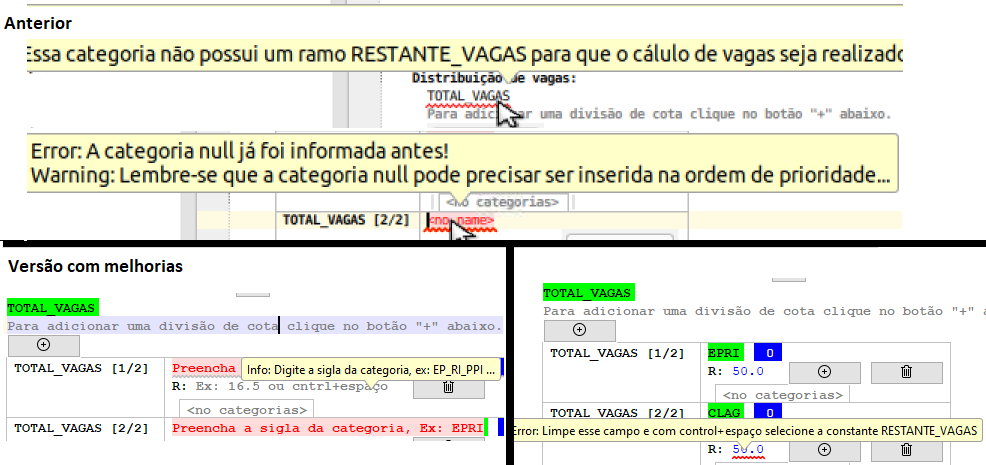
\includegraphics[width=0.94\textwidth]{chapters/analise/imagens/mensagens.png}}

\par\medskip\textbf{Fonte:} Elaborado pelo autor (2020). \par\medskip

\end{figure}



No que diz respeito às dificuldades dos usuários para seleção das categorias na seção \texttt{OrdemPrioridade}, foi alterado o editor para permitir adicionar novas categorias por meio do componente \texttt{JButton}, o qual facilita a seleção da categoria pelo usuário, sem precisar utilizar apenas o teclado para novas inclusões (Figura \ref{fig:melhoriaordem}). Destaca-se também, a modificação nas mensagens instrutivas sobre o preenchimento da ordem de prioridade, que deixaram de ser apresentadas em cada categoria da árvore de distribuição, para serem requisitadas apenas no momento de definição da ordem de prioridade.

\begin{figure}[ht!]
\centering

\caption{\textmd{Melhorias na seção Ordem de Prioridade}}
\label{fig:melhoriaordem}
\fcolorbox{gray}{white}{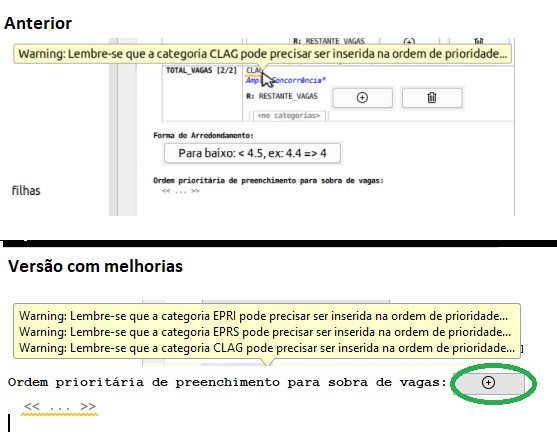
\includegraphics[width=0.94\textwidth]{chapters/analise/imagens/melhoriaordem.png}}

\par\medskip\textbf{Fonte:} Elaborado pelo autor (2020). \par\medskip

\end{figure}



Para tratar das dificuldades relatadas sobre o formato de preenchimento dos percentuais, foi alterada a regra de inferência dos elementos \texttt{Configuracao} e \texttt{CategoriaCota} para aceitar tanto valores inteiros como valores fracionados, evitando que o usuário tenha que preencher por exemplo "50.0". Isso foi possível pela comparação de tipagem fraca (\textit{weak subtype}) ao invés da comparação exata de tipos (\textit{strong subtype}).

\begin{figure}[ht!]
\centering

\caption{\textmd{Regra de inferência com \textit{weak sybtype}}}
\label{fig:weak}
\fcolorbox{gray}{white}{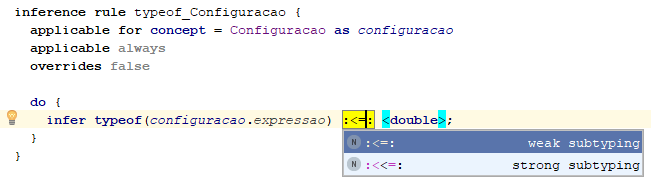
\includegraphics[width=0.75\textwidth]{chapters/analise/imagens/weark.png}}

\par\medskip\textbf{Fonte:} Elaborado pelo autor (2020). \par\medskip

\end{figure}



\newpage
As alterações descritas foram realizadas tendo como base as principais dificuldades apontadas pelos usuários da DSL. Desse modo, a versão final pode agregar valor ao presente estudo no que diz respeito ao uso de DSL como ferramenta de melhoria na comunicação entre os envolvidos, reduzindo eventuais incompreensões no uso da linguagem.

Na próxima Seção serão apresentados os resultados da análise com relação aos testes da \gls{API} DSL Cotas.